\documentclass{ubicomp-ext}
\usepackage{tikz}
\usepackage{float}
\usepackage{listings}
\usepackage{multicol}
\usepackage{color}
\usepackage{minibox}
\usepackage{fancybox}
\usepackage{fontspec}
\newfontfamily{\lstsansserif}[Scale=.625]{Arial}
\definecolor{Lemon}{HTML}{FFFACD}
\lstnewenvironment{csource}[1][]
    {\lstset{basicstyle=\lstsansserif,numberstyle=\numold,numbers=left,frame=lines,framexleftmargin=0.5em,framexrightmargin=0.5em,backgroundcolor=\color{Lemon},showstringspaces=false,escapeinside={(*@}{@*)},#1}}
    {}
% Please be sure that you have the dependencies (i.e., additional LaTeX packages) to compile this example.

\copyrightinfo{
  Copyright is held by the author/owner(s).\\
  {\emph{UbiComp '13 Adjunct}}, Sept 8-12, 2013, Zurich, Switzerland.\\
  ACM 978-1-4503-2139-6/13/09...\$15.00.
}

\title{Bringing Context-Oriented Programming into Embedded Systems}

\numberofauthors{8}
% Notice how author names are alternately typesetted to appear ordered in 2-column format;
% i.e., the first 4 autors on the first column and the other 4 auhors on the second column.
% Actually, it's up to you to strictly adhere to this author notation.
\author{
  \vspace{-1.5em} % lisatolles: The abstract heading should start at the time height on the page as the authors names
  \alignauthor{
  	\textbf{First Author}\\
  	\affaddr{AuthorCo, Inc.}\\
  	\affaddr{123 Author Ave.}\\
  	\affaddr{Authortown, PA 54321 USA}\\
  	\email{author1@anotherco.com}
  }\alignauthor{
  	\textbf{Fifth Author}\\
  	\affaddr{AuthorCo, Inc.}\\
  	\affaddr{123 Author Ave.}\\
  	\affaddr{Authortown, PA 54321 USA}\\
  	\email{author5@anotherco.com}
  }
  \vfil
}

% Paper metadata (use plain text, for PDF inclusion and later re-using, if desired)
\def\plaintitle{UbiComp 2013 LaTeX Extended Abstracts Template}
\def\plainauthor{Luis A. Leiva}
\def\plainkeywords{Guides, instructions, author's kit, conference publications}
\def\plaingeneralterms{Documentation, Standardization}

\hypersetup{
  % Your metadata go here
  pdftitle={\plaintitle},
  pdfauthor={\plainauthor},  
  pdfkeywords={\plainkeywords},
  pdfsubject={\plaingeneralterms},
  % Quick access to color overriding:
  %citecolor=black,
  %linkcolor=black,
  %menucolor=black,
  %urlcolor=black,
}

\usepackage{graphicx}   % for EPS use the graphics package instead
\usepackage{balance}    % useful for balancing the last columns
\usepackage{bibspacing} % save vertical space in references


\begin{document}

\maketitle

\begin{abstract}
Programming for embedded systems makes a significant part in the modern software development. Despite the rapid growth of the high-level languages there are still a necessity to use embedded systems. The prime example of this are Wireless Sensor Networks (WSNs). Most of the platforms for them are embedded.

The main task of WSNs is to monitor the environment. Thus, they are widely applied in different areas, such as health monitoring, wildlife tracking, smart home etc. But the environment is changing very fast, so it is necessary to react to these changes. In order to make WSN to be aware of changes we have to use a representation of the state of the environment within the WSN. In other words, we have to use \textit{Context} in programming for WSNs.

\textit{Context} could be defined as an entity, which represents a state of the environment. It can be used as a simplified model of the environment and could be formed according to sensing data. It is possible to develop more autonomous and more flexible system by using \textit{Contexts} in programming for WSNs.

Context-oriented programming (COP) is a programming technique which makes it possible to create an adaptive software by using \textit{Context} as an information about the state. Such a software could adapt to changes in the environment and to evolve according to this changes. The term ``evolve'' means that software can change behaviour and this behaviour depends on the context in which it is executed.

In this work we show how COP could be used for programming for embedded platforms and for WSNs in particular. We overview an example of the possible application of the WSN, then we extract the structure of the context for this application to highlight the specific aspects of the context-oriented approach in embedded systems. In the end we propose a small extension of the existing language for WSNs.
\end{abstract}
% =============================================================================
\section{Introduction}
% =============================================================================
Embedded systems are widely used to build different kind of devices and composition of devices. For example, in WSNs embedded platforms are mostly used. WSNs are inherently environment dependent. It  means that a programmer should always care about changes in data acquired by sensors. It leads to increasingly complex source-code. Even by using a representation of the state of the environment, it is hard to avoid complexity without elaborated tool. Thus it is hard to implement and maintain such a software.

In most cases WSNs are used as a passive components to gather data and to send it to the base station, where it is precessed. But there are also cases when WSN could be out of the range of the base station for a long period of time. In that case WSN should handle the changes in the external state (like changes in environment) and in the internal state (like exceptions within the program). In other words, WSN should be more autonomous and adaptive.

Context-Oriented Programming (COP) \cite{hirschfeld08} is an approach which provides an opportunity for a programmer to develop a software which can dynamically change the behaviour depending on context conditions. Context can be defined as ``any information that can be used to characterize the situation of an entity, where an entity can be a person, place or physical object" \cite{dey99}. Context-awareness can be defined as detecting current internal or external state of WSNs.

Context-Oriented Programming could be used as an effective way to use a \textit{Context} as a representation of the environment. It also will help to avoid the increasing complexity of a program. But bringing COP into embedded systems is accompanied by following challenges.

\begin{itemize}\compresslist
\item
While COP could provide a convenient way to use an environment representation in WSNs, the context structure for WSNs could be very complex and have non-trivial interaction. Thus, initial Context-Oriented paradigm could not be applied as is.
\item
Embedded platforms are mostly static, there are no tools for object-oriented or dynamic programming. Therefore, COP approaches for high-level languages (like Java, C++ or Python) are not applicable. 
\item
Embedded platforms also have restrictions on a hardware level, such as low memory, power consumption constraints, low performance.
\end{itemize}

Let's consider a simple example of the application of a WSN. 

Figure \ref{fig:shd} shows a state diagram of possible contexts of \textit{Smart Home}. In this application three classes could be found: \textit{Emergency} class, \textit{Location} class and \textit{Climate} class. Contexts of \textit{Emergency} class are activated if system detects intruders, fire or health emergency. There is a necessity to perform particular actions during context transition. For example, to call the police, the fire or an ambulance. \textit{Location} class includes \textit{outdoor} and rooms in house. During context transitions within \textit{location} class, system have to turn on/off lights and lock/unlock door. \textit{Climate} class could contains temperature contexts. If system detects high or low temperature, then it enables conditioner or heater.

\marginpar{
  \begin{figure}
    \centering
    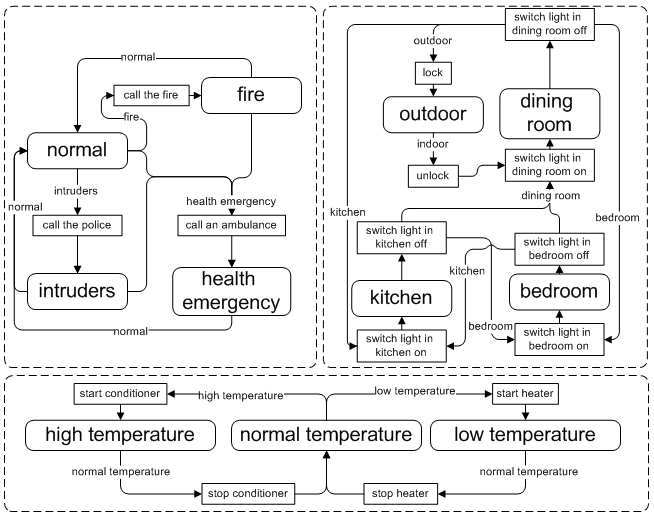
\includegraphics[width=\marginparwidth]{smarthome.png}
    \caption{Insert a caption below each figure.}
    \label{fig:shd}
  \end{figure}
}

\begin{Sbox}
\begin{minipage}{\marginparwidth}
\begin{csource}
(*@\textbf{context}@*) High {
 (*@\textbf{transitions}@*) Normal;
 uses interface Leds;
}
implementation {
 event void activated(){}
 event void deactivated(){}
 bool check(){return TRUE;}
 (*@\textbf{layered}@*) void toggle_leds(){
  call Leds.set(1);
 }
}
\end{csource}
\end{minipage}
\end{Sbox}

\marginpar{
  \begin{figure}
    \TheSbox
    \caption{Insert a caption below each figure.}
    \label{fig:shd}
  \end{figure}
}


\paragraph{Emergency class.} If WSN detects fire or housebreaking it can send an emergency call. If integrated with \textit{Healthcare system}, it can also activate emergency depends on \textit{Healthcare system} context. For example, if a householder has an injury or heart attack, the WSN can also activate a context from \textit{emergency} class.

\paragraph{Householder's location.} WSN can also track a householder's location. For example, if a householder moves from a kitchen to a dining room, the system switches off the light in the kitchen and switches on the light in the dining room. In this context system is also able to detect housebreaking. For example, if an unrecognized person appears in the house, while a householder is sleeping, then WSN activates the \textit{emergency} context. If a householder leaves the house, then \textit{Smart Home} could just lock the door. If a householder is nearby, then it could open the door.

\paragraph{Health monitoring.} WSN can be programmed to detect specific conditions and activate a specific context. For example, if the temperature in the room is lower (or higher) than normal, system can enable air heating (or conditioning) to return the temperature to the normal state. If \textit{Healthcare System} is integrated to \textit{Smart Home}, so the system can notify the householder about his current condition and recommend activities to improve householder's state of health.

But contexts can be divided into groups and considered as classes of contexts. Such classification brings COP on a new level of abstraction and makes it possible to operate complex structures of contexts as a superposition of smaller substructures. It also simplify the integration between different platforms, since another platform could be considered as a new class.

% =============================================================================
\section{ConesC}
% =============================================================================
We are using TinyOS and nesC language for demonstration purposes. In order to use context-oriented paradigm, we added new key-words in the language. We are also extended components by \textit{context} and \textit{context configuration}. \textit{Context} is an analog of \textit{module} and \textit{context configuration} is an analog of \textit{configuration}. These two components can be used as other components in nesC language.

\textit{Context} components is used to define context, possible transitions, actions before activation and after deactivation, layered functions, and to check transition conditions. In the rest it can be used like a \textit{module}.

On the figure \ref{fig:cc} context definition is displayed. Key word \textit{transitions} on the line 2 define legal transitions from context \textit{High}. It means, that only \textit{Normal} can be activated as the next context after \textit{High}. This definition is not mandatory. If \textit{transitions} are not defined, any transitions are legal. Line 3 represents regular nesC key word and means, that we are using \textit{Leds} component. Event \textit{activated} (line 6) is fired just before context activation, while event \textit{deactivated} (line 8) is fired just after deactivation. These events are also not mandatory. Method \textit{check()} represents \textit{context event check}. This method is called to verify conditions of context activation. If \textit{check()} returns FALSE, context will not be activated. If method is not defined, conditions will not be verified. Key-word \textit{layered} (line 13) indicates implementation of the function, which is specific for the current context. \textit{Layered} functions implementation is mandatory if they are defined in context configuration.

In the \textit{context} component \textit{context transition check} and \textit{context transition trigger} can also be specified. For example, on the line 2 (figure \ref{fig:ctre}) key-word \textit{while} declares, that transition from \textit{Indoor} to \textit{Outdoor} context can be activated only if \textit{Activity.Moving} context is active, where \textit{Activity} is a context class.

\begin{Sbox}
\begin{minipage}{\marginparwidth}
\begin{csource}
(*@\textbf{context configuration}@*) Temperature {
 (*@\textbf{layered}@*) void toggle_leds();
}
implementation {
 (*@\textbf{contexts}@*) High, 
  Normal (*@\textbf{is default}@*),
  Low;
 components LedsC;
 High.Leds -> LedsC;
 Normal.Leds -> LedsC;
 Low.Leds -> LedsC;
 Error.Leds -> LedsC;
}
\end{csource}
\end{minipage}
\end{Sbox}

\marginpar{
  \begin{figure}
    \TheSbox
    \caption{Insert a caption below each figure.}
    \label{fig:shd}
  \end{figure}
}

\begin{figure}
\begin{lstlisting}
context Indoor {
  transitions Outdoor while Activity.Moving;
}
implementation {
}
\end{lstlisting}
\caption{Context transition rule example.}
\label{fig:ctre}
\end{figure}

Programmer can also specify \textit{Context transition trigger} within the \textit{context} declaration. For example, if we have integration between two WSNs \textit{Smart Home} and \textit{Health Care}, programmer may want to activate \textit{SamrtHome.Emergency} context if \textit{HealthCare.Emergency} context was activated. It can be done as it shown on the line 2 of the figure \ref{fig:ctre}.

\begin{figure}[H]
\begin{lstlisting}
context Emergency {
  triggers SmartHome.Emergency;
}
implementation {
}
\end{lstlisting}
\caption{Context transition trigger example.}
\label{fig:ctre}
\end{figure}

\textit{Context configuration} component is used to define layered functions and context configuration. In the rest it can be used like a regular \textit{configuration}.

\begin{figure}
\begin{lstlisting}
context configuration Temperature {
  layered void toggle_leds();
}
implementation {
  contexts High,
    Normal is default,
    Low;
  components LedsC;
  High.Leds -> LedsC;
  Normal.Leds -> LedsC;
  Low.Leds -> LedsC;
  Error.Leds -> LedsC;
}
\end{lstlisting}
\caption{Context configuration component.}
\label{fig:ccc}
\end{figure}

In the listing \ref{fig:ccc} we assume, that contexts \textit{High}, \textit{Normal} and \textit{Low} are already defined. \textit{Error} context is default and generated by compiler, however it can be overridden by programmer in a standard context definition way. On the line 2 we declare a layered function, which should be implemented in each context. Lines 5, 6 and 7 show contexts belonging to the \textit{Temperature} class. It also indicates, that all declared contexts should implement layered functions. Line 6 also indicates that \textit{Normal} context will be active after initialization. The rest of the listing is a regular declaration of components and wires.

\textit{Context} and \textit{context configuration} has nesC-like structure and utilize the same logic. Both components can be used in native nesC way as a regular components.

\begin{figure}
\begin{lstlisting}
module DemoC {
  uses context configuration Temperature;
  uses interface Boot;
}
implemetation {
  event vois Boot.booted() {
    activate Temperature.Low;
    call Temperature.toggle_leds();
  }
  event void Temperature.contextChanged(context_t con) {
  }
}
\end{lstlisting}
\caption{Components usage example.}
\label{fig:cue}
\end{figure}

Figure \ref{fig:cue} displays a simple example. Here we declare, that we are using \textit{context configuration Temperature} (line 2). Key-word \textit{activate} (line 7) is used to activate a particular context in a particular context class. Here we activate context \textit{Low} of the context class \textit{Temperature}. Then we call a layered function (line 8). Behavior of the layered function depends on the activated context. Event \textit{contextChanged()} (line 10) is fired if the context within the particular context class has been changed.

\begin{figure}
\begin{lstlisting}
Configuration DemoAppC {
}
implementation {
  components
    Temperature,
    MainC,
    DemoC;
  DemoC.Temperature -> Temperature;
  DemoC.Boot -> MainC;
}
\end{lstlisting}
\caption{Components usage example (configuration).}
\label{fig:cuec}
\end{figure}

On the figure \ref{fig:cuec} main configuration is displayed. Here (lines 5 and 8) we use context configuration \textit{Temperature} as a regular component.

% =============================================================================
\section{Future work}
% =============================================================================
In the previous section we introduced new components and key words in the nesC language, but modifications are very slight and very well fitted. As one can notice, we made very slight changes in native nesC, but extended capabilities of the language. We also can notice strong rules in translation, which can be used to implement source-to-source compiler. In future work we will focus on the source-to-source compiler.

% =============================================================================
\section{Related Work}
% =============================================================================
The techniques for context-oriented programming were reviewed in details by Slavaschi et al. \cite{salvaneschi12}. Some of the techniques were utilized in the implementation of the COP in NesC.

In NesC there are no tools for dynamic loading and for object-oriented programming, so it is not possible to use \textit{in-laguage approach}, thus we are using \textit{source-to-source compiler} as it was proposed in \cite{salvaneschi12}. We are also using an idea of \textit{Layer in class}\cite{salvaneschi12}. However, there are no classes in NesC, so the idea was slightly chaged to fit the language restrictions. In context-oriented NesC each \textit{context} in \textit{context group} provides different implementation of layered functions. Also, several \textit{context groups} could provide the different sets of layers. Thus we define a set of layers within the one \textit{context group} to provide a behavioral variation.

In context NesC a modification of \textit{per-object} activaton method is used. This method also was reviewed in \cite{salvaneschi12}. But instead of objects there are \textit{components} in NesC. Thus activation occurs within the one component, which represents a \textit{context group}. This type of activation allows to keep a behavioral consistency, while adding behavioral variation.

This work was also partially inspired by \cite{kamina11}, where event-based context activation and context transitions were proposed. But there are also main differences, which makes this work original in the area.

While in \cite{kamina11} and \cite{kamina10} authors were focused on Java-based platforms and object-oriented languages, we are focused on embedded programming and on mobile WSNs particularly. In this work we consider embedded software platforms, which are usually characterized by restricted capabilities and limited resources. Thus, specific for WSNs optimization and adaptation should be performed. We also should to take into account the sensed data.

In \cite{kamina11} \textit{event declaration} and \textit{layer transition rules} were proposed. Considering \textit{layer} as a \textit{context}, we can ephasize another significant difference. While in \cite{kamina11} rules are only considered as activators and deactivators of the contexts, this work divide the term \textit{rule} into \textit{check} and \textit{trigger}. We also consider not only \textit{context transition} but also \textit{context event}, in other words, \textit{events} are expanded to cover the impact of the sensed data in WSNs. Thus we extend constructs proposed in \cite{kamina11}.



\section{Conclusion}
In this paper we discussed several WSNs applications and proposed possible contexts for different scenarios. Software for mobile WSNs becomes more complex, which makes it difficult to implement and to maintain. COP is intended to make a software  for WSNs more adaptable and less complex. We extracted different contexts within different scenarios and showed that COP could be used in applications for WSNs. We also considered context detection and possible behavior of the software within the particular context. This is  the first step to bringing COP to the programming for WSNs.

But even after extracting contexts, we can see a very complex structure and interactions between contexts. Complicity could be reduced by contexts classification. Moreover, classification makes it possible to provide integration between platforms easier: we can consider other platform as a separate class of contexts. For example, \textit{Smart home} could extract \textit{Healthcare} contexts to adapt home environment or to enable emergency. We also showed a necessity of defining a behavior not only within particular context, but also when transition between contexts occurs. There are also restrictions in context transitions, which also should be defined. Thus, COP for embedded programming should provide mechanisms of defining context classification, transitions and restrictions.

While transitions and restrictions are already proposed in \cite{kamina10} and can be implemented by event-based COP, context classification is not yet proposed. Classification, context transitions and restrictions could make platform integration and programming for WSNs easier and more effective.

We are also proposed a language extension for nesC, which introduces new key-words and types of components. As shown in this paper, our approach not only extend language capabilities, but also simplify developing process by generating the source code. 

\balance
\bibliographystyle{acm-sigchi}
\bibliography{ubicomp}

\end{document}